\documentclass[letterpaper, 10pt]{article}
\usepackage{amsmath} %For math notation
\usepackage{amssymb} %For symbols/fonts used in math
\usepackage{tikz} %For diagrams/nodes
\usepackage{longdivision} %For long division
\usepackage{tkz-euclide} %For euclidean geometry
\usepackage{pgfplots}
\usepackage[margin=1in]{geometry} %for page setup

\author{Jacob Seadorf}
\title{Pre-Algebra Math Notes}
\graphicspath{{./images/}}

\begin{document}
\maketitle
\section{Whole Numbers}
	Whole numbers are all numbers without fractions, and is a collection of positive integers and zero. Whole numbers are represented in math by $\mathbb{W}$. Some examples of whole numbers include (but are not limited to): $0, 12, 456, 45,762$.

	\subsection{Properties of Whole Numbers}
	Whole numbers have certain properties:
	
	\textbf{Addition}:
	\begin{itemize}
		\item Addition Property of 0: $a + 0 = a$ and $0 + a = a$
		\item Commutative Property of Addition: $a + b = b + a$
		\item Associative Property of Addition: $(a + b) + c = a + (b + c)$
	\end{itemize}
	
	\textbf{Multiplication}:
	\begin{itemize}
		\item Property of Zero: $a \times 0 = 0$ and $0 \times a = 0$
		\item Commutative Property: $a \times b = b \times a$
		\item Associative Property: $(a \times b) \times c = a \times (b \times c)$
		\item Property of 1: $a \times 1 = a$ and $1 \times a = a$
		\item Distributive Property: $a(b + c) = (a \times b) + (a \times c)$
	\end{itemize}

	\textbf{Division}:
		\begin{itemize}
		\item $a \div 0 = undefined$
		\end{itemize}
\section{Order of Operations}
	The order of how you solve an equations matters; if you get the order wrong, you get the wrong answer. An easy way to remember the order of operations is the acronym ``PEMDAS'' (Parenthesis, Exponents, Multiplication, Division, Addition, Subtraction). 



\textbf{Remember}: A negative times a negative equals a positive; a positive times a negative equals a negative
	\subsection{Examples}
		\subsubsection{Example 1}
		$$17 + 3(7-\sqrt{9})^2 $$
		$$17 + 3(7 - 3)^2 $$
		$$17 + 3 (4)^2$$
		$$17 + 3(16)$$
		$$17 + 48$$	
		$$65$$
\section{Absolute Value}
	 For any number $a$, $|a|$ is the distance between $a$ and 0 on the number line.
	\subsection{Examples}
	\subsubsection{Example 1}
	$$
	|-8| = 8
	$$
	\subsubsection{Example 2}	
	$$
	|16| = 16
	$$
\section{Algebraic Expressions \& Like Terms}
\textbf{Terms}: Numbers or variables used in addition or subtraction problems.

Example: $$2x + 3$$

\noindent \textbf{Like Terms}: A term with the same variable or exponent as another term.

Example: $$3x^2, 4x^2$$


\subsection{Examples}
\subsubsection{Example 1}
$$5(3 + w)$$
$$5(3) + 5w$$
$$15 + 5w$$

\subsubsection{Example 2}
$$14a - 5b + 3a - b - 3$$
$$14a + 3a - 5b - b - 3$$
$$17a - 6b - 3$$

\subsubsection{Example 3}
$$16p - 3 (2p - q) + 7q$$
$$16p - 6p + 3q + 7q$$
$$10p + 10q$$


\section{Algebraic Equations}
We've already looked at algebraic \textit{expressions}, but what's the difference between an expression and an equation? An equals sign. 

\textbf{Solve}: To find the value(s) that make an equation true.

To solve an equation, think ``what are you undoing in order to get the variable by itself?''

\subsection{Examples}
\subsubsection{Example 1}
	$$3y - 2 = 4$$
	Is 2 a solution? 
	$$3(2) - 2 = 4$$
	$$6 - 2 = 4$$
	Yes, 2 is a solution.


\subsubsection{Example 2}
$$y - 12 = 30$$
Add 12 to both sides (you're undoing subtraction).
$$y = 42$$

\section{Fractions \& Mixed Numbers}
\subsection{Rules for Fractions}
$$
\frac{a}{1} = a
$$

$$
\frac{a}{a} = 1
$$

$$
\frac{0}{a} = 0
$$

$$ 
\frac{a}{0} = undefined
$$

$$
\frac{-a}{-b} = \frac{a}{b}
$$

\subsection{Mixed Numbers to Improper Fractions}
There's two steps: 
\begin{enumerate}
\item Multiply denominator by whole number.
\item Add result to numerator.
\end{enumerate}

\subsection{Examples}
\subsubsection{Example 1}
$$
6\frac{1}{3}
$$

$$
\frac{19}{3}
$$

\subsection{Improper Fractions to Mixed Numbers}
There's only two steps to creating an improper fraction from a mixed number: 
\begin{enumerate}
\item Divide numerator by denominator.
\item Quotient is the whole number; remainder is the numberator.
\end{enumerate}

\subsection{Examples}
\subsubsection{Example 1}
$$
-\frac{43}{18}
$$

$$
43 \div 18 = 2R7
$$

$$
-2\frac{7}{18}
$$

\section{Simplifying Fractions}
\noindent \textbf{Simplified Fraction}: When the numerator and denominator have no common factors and both numbers are whole.

\subsection{Examples}
\subsubsection{Example 1}
$$
\frac{15}{18}
$$
Divide both the numerator and denominator by 3 (the common factor between 15 and 18).

$$
\frac{5}{6}
$$


\section{Fraction Multiplication \& Division}
\noindent \textbf{Reciprocal}: 1 divided by a number (or a number raised to the power of -1). Think of it like the fraction is standing on its ``head'' (numerator).


To multiply fractions, I would recommend simplifying first, then multiplying.

To divide fractions, multiply by the reciprocal

$$
\frac{a}{b} \times \frac{c}{d} = \frac{ac}{bd}
$$

$$
\frac{a}{b} \div \frac{c}{d} = \frac{a}{b} \times \frac{d}{c}
$$
\subsection{Examples}
\subsubsection{Example 1}
	$$
	\frac{3ab}{7} \div \frac{15a}{14}
	$$

	$$
	\frac{3ab}{7} \times \frac{14}{15a} = \frac{2b}{5}
	$$


\section{Fraction Addition \& Subtraction}
To add or subtract fractions, we \textbf{must} have a common denominator!

$$
\frac{a}{c} \pm \frac{b}{c} = \frac{a \pm b}{c}
$$

\subsection{Examples}
\subsubsection{Example 1}
$$
\frac{1}{21} + \frac{13}{21} = \frac{14}{21}
$$
Simplifying (by dividing by 7)...
$$
\frac{2}{3}
$$

\subsubsection{Example 2}
$$
\frac{11a}{4b} + \frac{7}{4b} = \frac{11a + 7}{4b}
$$

\section{Order of Operations with Fractions}
\subsection{Examples}
\subsubsection{Example 1}
	$$
	\left(-\frac{1}{4}\right)^2 \Rightarrow 
	\left(-\frac{1}{4}\right) \left(-\frac{1}{4}\right) 
	= \frac{1}{16}
	$$
\subsubsection{Example 2}
	$$
	\frac{-4}{5}p + \frac{2}{5}p = \frac{-2}{5}p
	$$

\subsection{Example 3}
	$$
	\frac{1}{3}b + \frac{2}{9}b
	$$
	We need a common denominator to add fractions; the least common denominator is 3.

	Multiply one of the fractions by the least common denominator to ``build up'' a fraction.
	$$
	\frac{3}{3} \times \frac{1}{3}b \Rightarrow \frac{3}{9}b + \frac{2}{9}b = \frac{5}{9}b
	$$

\section{Solving Equations with Fractions}
\subsection{Examples}
\subsubsection{Example 1}
	$$
	x - \frac{3}{10} = \frac{9}{20}
	$$

	Isolate the variable...
	$$
	x = \frac{9}{20} + \frac{3}{10}
	$$
	The least common denominator is 2; build up the fraction...
	$$
	\frac{3}{10} \times \frac{2}{2} = \frac{6}{20}	
	$$

	Add the fractions...
	$$
	x = \frac{9}{20} + \frac{6}{20} \Rightarrow x = \frac{15}{20}
	$$
	Reduce the fraction...	

	$$
	x = \frac{3}{4}
	$$

\section{Ratios}
\noindent \textbf{Ratio}: The quotient of 2 quantities with the \underline{same} units.
There's three ways to write ratios: $\frac{a}{b}$, $a$ to $b$, $a : b$.
\subsection{Examples}
\subsubsection{Example 1}
A recipie calls for 3 cups of flour and 2 cups of milk for one person; how many cups of each would you need for 4 people?

The ratio is $ 3 : 2$, because for every 3 cups of flour, we need 2 cups of milk.

$$
\frac{3}{2} \times \frac{4}{4} = \frac{12}{8}
$$
To make the recipie for 4 people, you would need 12 cups of flour and 8 cups of milk.

\section{Rates}
\textbf{Rate}: The quotient of 2 quantities with \underline{different} units.

\noindent \textbf{Unit Rate}: A rate with a denominator of 1.

To find a unit rate, divide the numerator by the denominator, and keep the units. 
\subsection{Examples}
	\subsubsection{Example 1}
	There are 50 students to 4 advisors; how many students are there to 2 advisors? 
	$$
	\frac{50}{4} \div \frac{2}{2} \Rightarrow \frac{25}{2}
	$$
	\subsubsection{Example 2}
	A home-improvement store sells a bag of 12 tiles for \$13.08; what is the price per tile?
	$$
	\frac{\$13.08}{12} = \frac{\$1.09}{tile}
	$$

	\subsubsection{Example 3}
	3 shirts cost \$64.80; what is the price of one shirt?
	$$
	\frac{\$64.80}{3} = \frac{\$21.60}{shirt}
	$$

\section{Simple \& Compound Interest}
\subsection{Simple Interest Formula}
$$I = Prt, A = P+I$$
\noindent \begin{tabular}{|c|c|c|c|c|}
	\hline
	I & P & r & t & A \\
	Interest & Principal & annual interest rate & time, in years & total amount in account \\ 
	\hline
\end{tabular}

\subsection{Compound Interest Formula}
$$A = P\left(1 + \frac{r}{n}\right)^n^t$$
\noindent \begin{tabular}{|c|c|c|c|}
	\hline
	P & r & n & t \\
	Principal & annual nominal interest rate & number of times compounded/year & number of years \\
	\hline
\end{tabular}

\section{Pythagorean Theorem \& Triangles}

For any right triangle (see the picture below), you can find the length of the hypotenuse with the Pythagorean Theorem: $a^2 + b^2 = c^2$

\noindent \textbf{Hypotenuse}: The longest side of a right triangle, usually labeled as $c$.

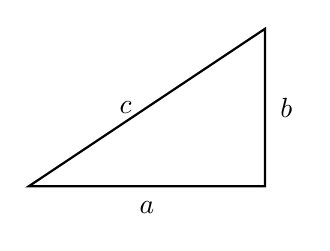
\begin{tikzpicture}
%Triangle coordinates so I don't have to enter the coordinates every time
\coordinate (P) at (1,1);
\coordinate (Q) at (4,1);
\coordinate (R) at (4,3);

%Drawing the triangle
\draw[thick] (P)--(Q)--(R)--cycle;

\tkzLabelSegment[below=2pt](P,Q) {$a$}
\tkzLabelSegment[right=2pt](R,Q) {$b$}
\tkzLabelSegment[left=2pt](P,R) {$c$}
\end{tikzpicture}

\subsection{Examples}
\subsubsection{Example 1}

For a right triangle with side lengths of 7 and 24 centimeters, find the length of side $c$.
$$
7^2 + 24^2 = c^2
$$

$$
49 + 576 = c^2
$$

$$
625 = c^2
$$

$$
\sqrt{625} = 25 cm
$$

\section{Two Variable Linear Equations}
The standard form for a linear equation is: 
	$$
	ax + by = c
	$$

\noindent \textbf{X-intercept}: The point where the line on a coordinate plane crosses the x-axis $(x,0)$.

\noindent \textbf{Y-intercept}: The point where the line on a coordinate plane crosses the y-axis $(0,y)$.

\subsection{Examples}
\subsubsection{Example 1}
$$2x + 3y = 6$$
\textbf{Finding the X-intercept}:
$$2x + 3(0) = 6$$

Anything multiplied by 0 equals 0, so remove it from the equation...
$$2x = 6$$
Divide both sides by 2...
$$x = 3$$
The X-intercept is (3,0).

\textbf{Finding the Y-intercept}:
$$2(0) + 3y = 6$$
Solve for y...
$$3y = 6$$
Divide by 3...
$$y = 2$$
The Y-intercept is at (0,2)

\end{document}
